
\chapter{Gauss Integrals}
\label{appendix:gauss_integrals}
The protein backbone is a curve in space. One well-known measure of how two curves interact is the Gauss integral, also called Gauss invariant. The generalized Gauss integrals originate in integral formulas of Vassiliev knot invariants \cite{Bar-Natan1995} and give absolute measures of protein geometry. The integrals may be understood as crossing numbers and correlations along the backbone of crossing numbers. Two of the simplest structural measures are considered: the writhe and the average crossing number. The writhe, $Wr$, of a closed space curve, $\gamma$, may be computed by using the Gauss integral
\begin{equation}
 Wr(\gamma) = \frac{1}{4\pi}\iint_{\gamma \times \gamma \backslash D} \omega(t_1, t_2)dt_1dt_2
\end{equation}
where $\omega(t_1, t_2) = [\gamma\ '(t_1), \gamma(t_1) - \gamma(t_2), \gamma\ '(t_2)] / |\gamma(t_1) - \gamma(t_2)|^3$, $D$ is the diagonal of $\gamma \times \gamma$, and $[\gamma\ '(t_1), \gamma(t_1) - \gamma(t_2), \gamma\ '(t_2)]$ is the triple scalar product. As $\omega(t_1, t_2) = \omega(t_2, t_1)$, the writhe may be calculated as an integral over a 2-simplex, namely
\begin{equation}
 I_{(1,2)}(\gamma) = Wr(\gamma) = \frac{1}{2\pi}\iint_{0 < t_1 < t_2 < L} \omega(t_1, t_2)dt_1dt_2
\end{equation}
For a polygonal curve $\mu$, the definition of the writhe is
\begin{equation}
 I_{(1,2)}(\mu) = Wr(\mu) = \sum_{0 < i_1 < i_2 < N} W(i_1, i_2)
\end{equation}
where $N$ is the size of the protein, with 
\begin{equation}
 W(i_1, i_2) = \frac{1}{2\pi}\int_{i_1 = t_1}^{i_1 + 1} \int_{i_2 = t_2}^{i_2 + 1} w(t_1, t_2)dt_1dt_2
\end{equation}
where $W(i_1, i_2)$ is the contribution to writhe coming from the $i_1$th and the $i_2$th line segments, which equals the probability to see the $i_1$th and the $i_2$th line segments cross from an arbitrary direction, multiplied by the sign of this crossing, see Figure \ref{fig:sphere_gi}. 
\begin{figure}[tb]
	\begin{center}
		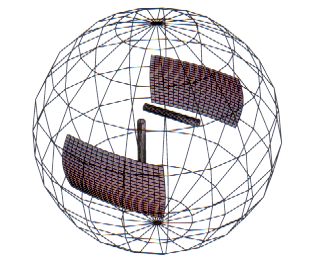
\includegraphics[scale=0.80]{sphere_gi}
		\caption[Gauss integrals and crossings]{On the unit sphere, the filled area corresponds to normals of planes in which the two projected line segments are seen to cross. The two line segments are seen to cross with a probability $|W|$ equal to the filled area divided by the area of the whole sphere when averaged over all directions in space. A positive crossing is seen ($W$ positive) whenever the line segment in the front is traversed upwards and the rear line segment is traversed from right to left or if both line segments are traversed in the opposite direction. Otherwise a negative crossing is seen ($W$ negative).}
		\label{fig:sphere_gi}
	\end{center}
\end{figure}
Geometrically, the writhe is the signed average number of crossings averaged over the observer's position located in all space directions. \\
The unsigned average number of crossings seen from all directions is known as the average crossing number and is defined as
\begin{equation}
 I_{|1,2|}(\mu) = \sum_{0 < i_1 < i_2 < N} |W(i_1, i_2)|
\end{equation}
A whole family of structural measures, defined over the second and third order Gauss invariants, e.g. 
\begin{equation}
 I_{|1,3|(2,4)}(\mu) = \sum_{\substack{0 < i_1 < i_2 \\ 
			     < i_3 < i_4 < N}} |W(i_1, i_3)|W(i_2, i_4)
\end{equation}
and
\begin{equation}
I_{(1,5)(2,4)(3,6)}(\mu) = \sum_{\substack{0 < i_1 < i_2 < i_3 \\ 
				< i_4 < i_5 < i_6 < N}} W(i_1, i_5)W(i_2, i_4)W(i_3, i_6)
\end{equation}
may be constructed by using writhe and average crossing number as the basic building blocks. The usefulness of the higher order invariants is that these can be able to distinguish curves which have the same writhe and average crossing number.\\
To understand better, a simple example is reported. Consider the axis of each tube in Figure \ref{fig:curves} to be given by a polygonal curve. 
\begin{figure}[tb]
	\begin{center}
		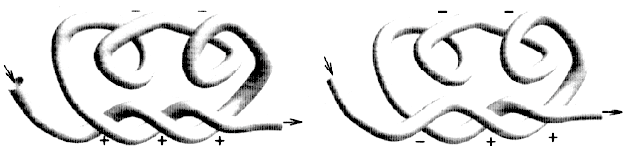
\includegraphics[scale=0.60]{curves}
		\caption[Two tubes with the signs of the crossings seen in this projection]{Two tubes with the signs of the crossings seen in this projection.}
		\label{fig:curves}
	\end{center}
\end{figure}
When the two tubes are pushed down to almost lie in the plane, the $W(i, j)$ in the formula tends either to $-1$, to $0$ or to $+1$. In fact, if the line segments $i$ and $j$ are seen to lie apart in the figure, then in the plane limit they will lie apart and in the same plane. The set of directions from which they are seen to cross will diverge to a set of two arcs with measure $0$ on the unit 2-sphere. That is, $W(i, j)$ tends to $0$. However, if the two line segments are seen to cross in the planar projection in which they are pushed into, then in the limit they are seen to cross from all direction on the unit 2-sphere. Hereby, $W(i, j)$, tends to $\pm1$ depending on the sign of the crossing. The writhe of the left tube in Figure \ref{fig:curves} is $I_{(1,2)}(W_{left}) \approx 3 \times (+1) + 2 \times (-1) = +1$ and that of the right tube is $I_{(1,2)}(W_{right}) \approx 2 \times (+1) + 3 \times (-1) = -1$, while the average crossing number is $\approx 5$ for both tubes due to ignoring the signs of crossings.


\cleardoublepage